\documentclass[11pt,a4paper]{article}
\usepackage[utf8]{inputenc}
\usepackage[margin=1in]{geometry}
\usepackage{graphicx}
\usepackage{tikz}
\usepackage{listings}
\usepackage{xcolor}
\usepackage{amsmath}
\usepackage{hyperref}
\usepackage{fancyhdr}
\usepackage{enumitem}

% TikZ libraries
\usetikzlibrary{shapes.geometric, arrows, positioning, fit, backgrounds}

% Code highlighting setup
\lstset{
    basicstyle=\ttfamily\small,
    keywordstyle=\color{blue},
    commentstyle=\color{green!60!black},
    stringstyle=\color{red},
    backgroundcolor=\color{gray!10},
    frame=single,
    breaklines=true,
    showstringspaces=false,
    numbers=left,
    numberstyle=\tiny\color{gray}
}

% Page header
\pagestyle{fancy}
\fancyhf{}
\fancyhead[L]{Book Service API}
\fancyhead[R]{Workflow Documentation}
\fancyfoot[C]{\thepage}

\title{\textbf{Book Service API}\\ \large{Workflow and Architecture Documentation}}
\author{TypeScript \& Express.js REST API}
\date{\today}

\begin{document}

\maketitle

\tableofcontents
\newpage

\section{Overview}
The Book Service API is a RESTful web service built with TypeScript and Express.js that provides comprehensive CRUD (Create, Read, Update, Delete) operations for managing a library system. The application uses JSON files for data persistence, making it lightweight and suitable for development and learning purposes.

\subsection{Key Features}
\begin{itemize}
    \item Authors management with biographical information
    \item Books management with multi-author support
    \item Relationship mapping between books and authors via IDs
    \item File-based JSON storage for simplicity
    \item Automatic ID generation and management
    \item Comprehensive error handling with proper HTTP status codes
\end{itemize}

\section{System Architecture}

\subsection{Project Structure}
The application follows a modular architecture with clear separation of concerns:

\begin{figure}[h]
\centering
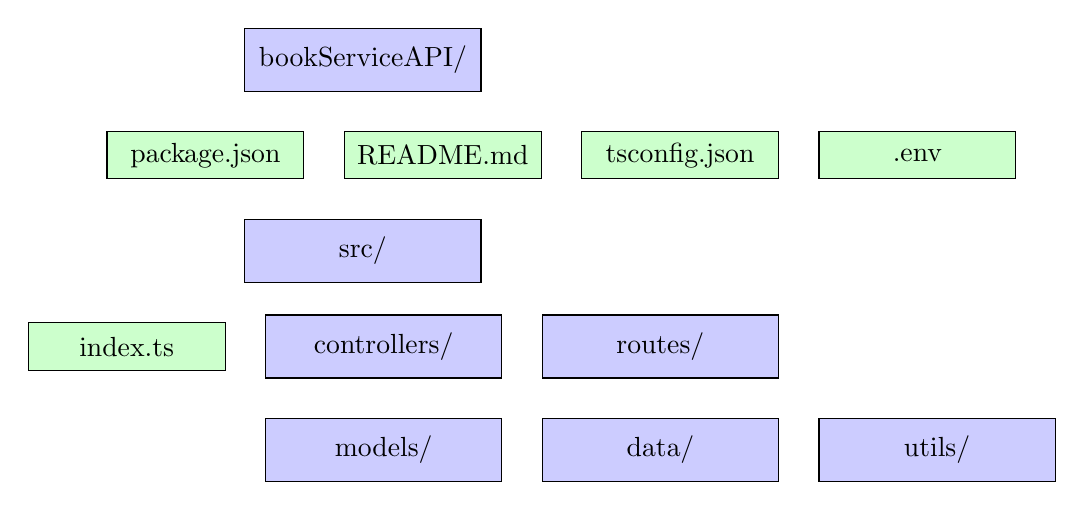
\begin{tikzpicture}[
    node distance=0.5cm,
    folder/.style={draw, rectangle, minimum width=3cm, minimum height=0.8cm, fill=blue!20},
    file/.style={draw, rectangle, minimum width=2.5cm, minimum height=0.6cm, fill=green!20}
]
    % Root folder
    \node[folder] (root) {bookServiceAPI/};
    
    % Main files
    \node[file, below=of root, xshift=-2cm] (package) {package.json};
    \node[file, right=of package] (readme) {README.md};
    \node[file, right=of readme] (tsconfig) {tsconfig.json};
    \node[file, right=of tsconfig] (env) {.env};
    
    % src folder
    \node[folder, below=of package, xshift=2cm] (src) {src/};
    
    % src contents
    \node[file, below=of src, xshift=-3cm] (index) {index.ts};
    \node[folder, right=of index] (controllers) {controllers/};
    \node[folder, right=of controllers] (routes) {routes/};
    \node[folder, below=of controllers] (models) {models/};
    \node[folder, right=of models] (data) {data/};
    \node[folder, right=of data] (utils) {utils/};
    
\end{tikzpicture}
\caption{Project Structure Overview}
\end{figure}

\subsection{Technology Stack}
\begin{itemize}
    \item \textbf{Runtime}: Node.js
    \item \textbf{Language}: TypeScript for type safety
    \item \textbf{Framework}: Express.js for web server
    \item \textbf{Development}: Nodemon for auto-reload
    \item \textbf{Data Storage}: JSON files for persistence
\end{itemize}

\section{Application Workflow}

\subsection{Request Processing Flow}

\begin{figure}[h]
\centering
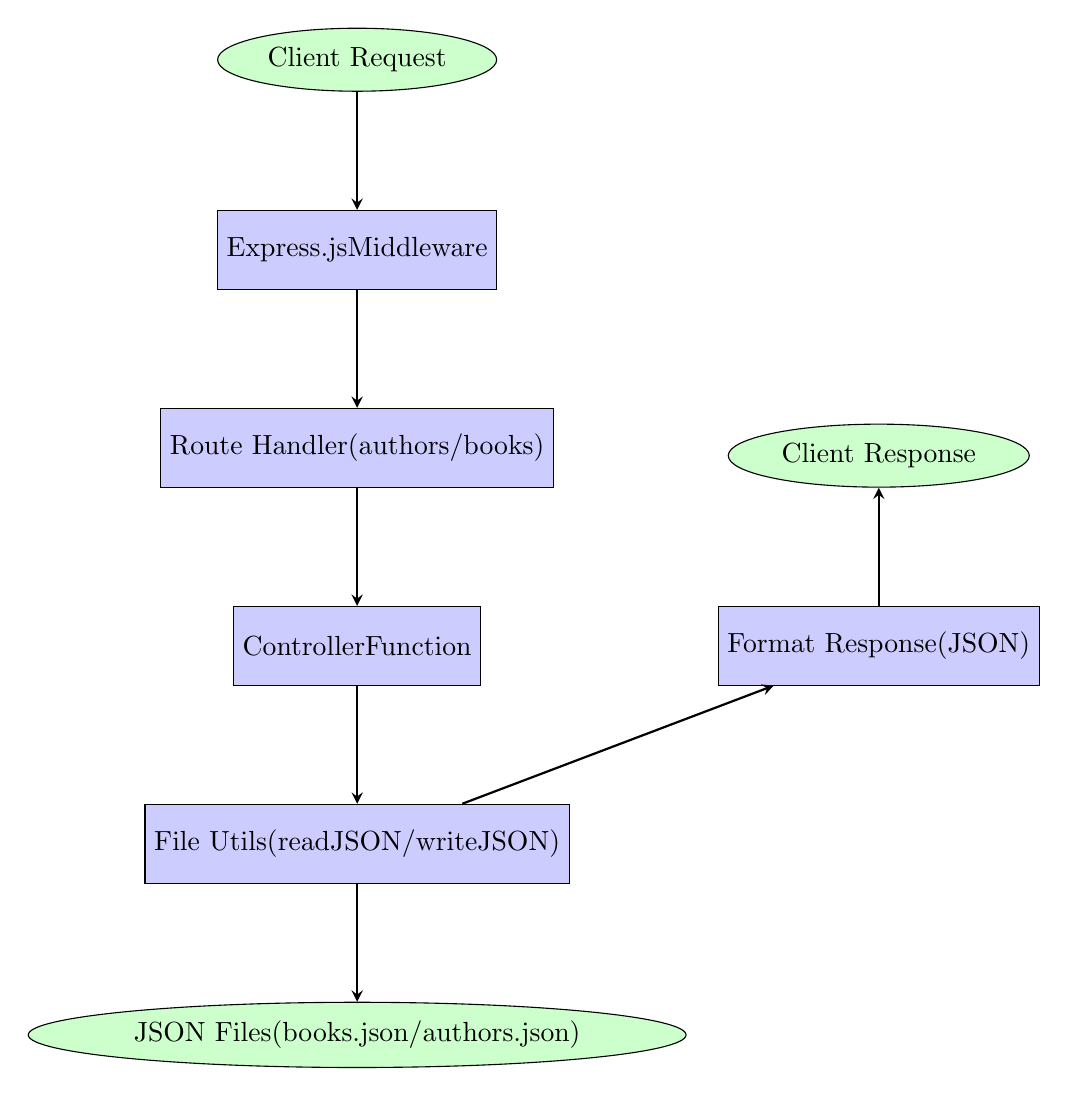
\begin{tikzpicture}[
    node distance=1.5cm,
    process/.style={rectangle, draw, fill=blue!20, minimum width=2.5cm, minimum height=1cm, text centered},
    decision/.style={diamond, draw, fill=yellow!20, minimum width=2cm, minimum height=1cm, text centered},
    data/.style={ellipse, draw, fill=green!20, minimum width=2cm, minimum height=0.8cm, text centered},
    arrow/.style={thick,->,>=stealth}
]
    % Start
    \node[data] (client) {Client Request};
    
    % Express middleware
    \node[process, below=of client] (express) {Express.js\\Middleware};
    
    % Routing
    \node[process, below=of express] (routing) {Route Handler\\(authors/books)};
    
    % Controller
    \node[process, below=of routing] (controller) {Controller\\Function};
    
    % File operations
    \node[process, below=of controller] (fileops) {File Utils\\(readJSON/writeJSON)};
    
    % JSON files
    \node[data, below=of fileops] (jsonfiles) {JSON Files\\(books.json/authors.json)};
    
    % Response
    \node[process, right=3cm of controller] (response) {Format Response\\(JSON)};
    
    % Client response
    \node[data, above=of response] (clientresp) {Client Response};
    
    % Arrows
    \draw[arrow] (client) -- (express);
    \draw[arrow] (express) -- (routing);
    \draw[arrow] (routing) -- (controller);
    \draw[arrow] (controller) -- (fileops);
    \draw[arrow] (fileops) -- (jsonfiles);
    \draw[arrow] (fileops) -- (response);
    \draw[arrow] (response) -- (clientresp);
    
\end{tikzpicture}
\caption{Request Processing Workflow}
\end{figure}

\subsection{Detailed Workflow Steps}

\begin{enumerate}
    \item \textbf{Client Request}: HTTP request arrives at Express server
    \item \textbf{Middleware Processing}: Express.js processes the request
    \begin{itemize}
        \item Parses JSON body using \texttt{express.json()}
        \item Extracts route parameters and query strings
    \end{itemize}
    \item \textbf{Route Matching}: Express router matches URL to appropriate handler
    \item \textbf{Controller Execution}: Specific controller function is called
    \item \textbf{Data Operations}: File utilities handle JSON file operations
    \item \textbf{Response Generation}: Data is formatted and sent back to client
\end{enumerate}

\section{CRUD Operations}

\subsection{Create Operation Workflow}

\begin{figure}[h]
\centering
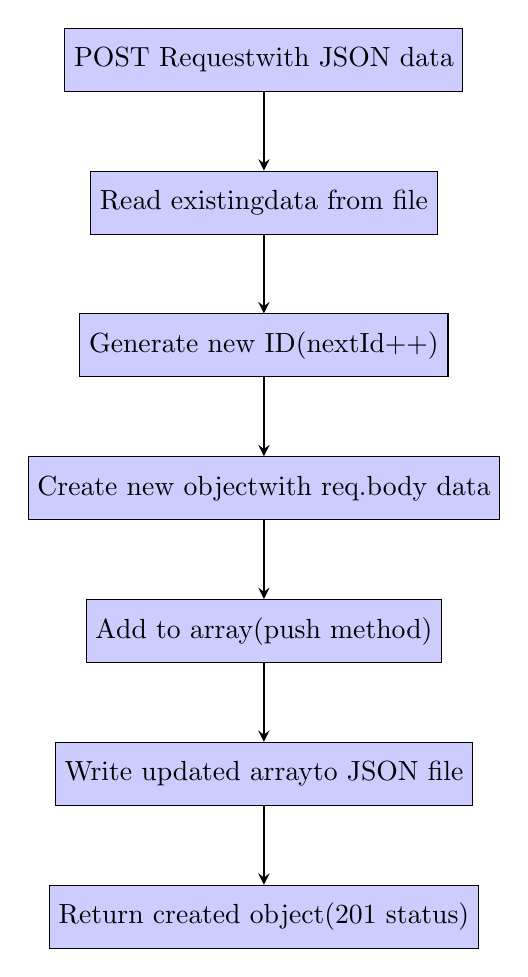
\begin{tikzpicture}[
    node distance=1cm,
    process/.style={rectangle, draw, fill=blue!20, minimum width=3cm, minimum height=0.8cm},
    decision/.style={diamond, draw, fill=yellow!20, minimum width=2.5cm, minimum height=0.8cm},
    arrow/.style={thick,->,>=stealth}
]
    \node[process] (start) {POST Request\\with JSON data};
    \node[process, below=of start] (read) {Read existing\\data from file};
    \node[process, below=of read] (generate) {Generate new ID\\(nextId++)};
    \node[process, below=of generate] (create) {Create new object\\with req.body data};
    \node[process, below=of create] (add) {Add to array\\(push method)};
    \node[process, below=of add] (write) {Write updated array\\to JSON file};
    \node[process, below=of write] (respond) {Return created object\\(201 status)};
    
    % Arrows
    \draw[arrow] (start) -- (read);
    \draw[arrow] (read) -- (generate);
    \draw[arrow] (generate) -- (create);
    \draw[arrow] (create) -- (add);
    \draw[arrow] (add) -- (write);
    \draw[arrow] (write) -- (respond);
\end{tikzpicture}
\caption{Create Operation Flow}
\end{figure}

\subsection{Update Operation Workflow}

\begin{figure}[h]
\centering
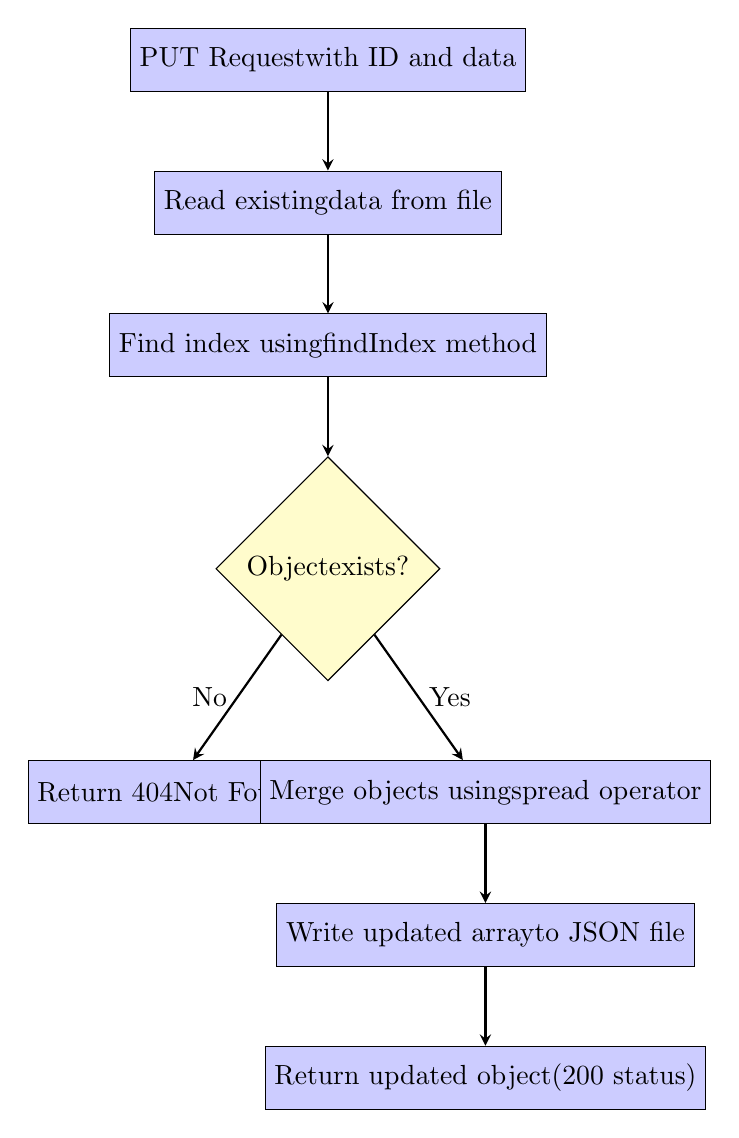
\begin{tikzpicture}[
    node distance=1cm,
    process/.style={rectangle, draw, fill=blue!20, minimum width=3cm, minimum height=0.8cm},
    decision/.style={diamond, draw, fill=yellow!20, minimum width=2.5cm, minimum height=0.8cm},
    arrow/.style={thick,->,>=stealth}
]
    \node[process] (start) {PUT Request\\with ID and data};
    \node[process, below=of start] (read) {Read existing\\data from file};
    \node[process, below=of read] (find) {Find index using\\findIndex method};
    \node[decision, below=of find] (exists) {Object\\exists?};
    \node[process, below=of exists, xshift=-2cm] (error) {Return 404\\Not Found};
    \node[process, below=of exists, xshift=2cm] (merge) {Merge objects using\\spread operator};
    \node[process, below=of merge] (write) {Write updated array\\to JSON file};
    \node[process, below=of write] (respond) {Return updated object\\(200 status)};
    
    % Arrows
    \draw[arrow] (start) -- (read);
    \draw[arrow] (read) -- (find);
    \draw[arrow] (find) -- (exists);
    \draw[arrow] (exists) -- node[left] {No} (error);
    \draw[arrow] (exists) -- node[right] {Yes} (merge);
    \draw[arrow] (merge) -- (write);
    \draw[arrow] (write) -- (respond);
\end{tikzpicture}
\caption{Update Operation Flow}
\end{figure}

\section{Code Structure Analysis}

\subsection{Controller Functions}

Each controller function follows a consistent pattern:

\begin{lstlisting}[language=JavaScript, caption=Generic Controller Pattern]
export const controllerFunction = (req: Request, res: Response): void => {
    // 1. Read current data from JSON file
    const data: Type[] = readJSON(FILE_PATH);
    
    // 2. Process request (find, create, update, delete)
    // Business logic specific to operation
    
    // 3. Write data back to file (if modified)
    writeJSON(FILE_PATH, data);
    
    // 4. Send appropriate response
    res.status(statusCode).json(responseData);
}
\end{lstlisting}

\subsection{Key Syntactic Elements}

\subsubsection{Object Spread Operator in Updates}
\begin{lstlisting}[language=JavaScript]
// Merge existing object with new data
books[index] = { ...books[index], ...req.body };
\end{lstlisting}

\subsubsection{Array Methods for Data Manipulation}
\begin{lstlisting}[language=JavaScript]
// Finding elements
const book = books.find(b => b._id === Number(req.params.id));
const index = books.findIndex(b => b._id === Number(req.params.id));

// Removing elements
const deleted = books.splice(index, 1);
\end{lstlisting}

\subsubsection{ID Generation Strategy}
\begin{lstlisting}[language=JavaScript]
// Initialize next ID based on existing data
let nextBookId = 1;
const existingBooks: Book[] = readJSON(BOOKS_FILE);
if(existingBooks.length > 0){
    const lastBook: Book = existingBooks[existingBooks.length - 1];
    nextBookId = lastBook._id + 1;
}
\end{lstlisting}

\section{API Endpoints}

\subsection{Authors API}
\begin{center}
\begin{tabular}{|l|l|l|}
\hline
\textbf{Method} & \textbf{Endpoint} & \textbf{Description} \\
\hline
GET & /authors & Retrieve all authors \\
GET & /authors/:id & Retrieve specific author \\
POST & /authors & Create new author \\
PUT & /authors/:id & Update existing author \\
DELETE & /authors/:id & Delete author \\
\hline
\end{tabular}
\end{center}

\subsection{Books API}
\begin{center}
\begin{tabular}{|l|l|l|}
\hline
\textbf{Method} & \textbf{Endpoint} & \textbf{Description} \\
\hline
GET & /books & Retrieve all books \\
GET & /books/:id & Retrieve specific book \\
POST & /books & Create new book \\
PUT & /books/:id & Update existing book \\
DELETE & /books/:id & Delete book \\
\hline
\end{tabular}
\end{center}

\section{Data Models}

\subsection{Author Model}
\begin{lstlisting}[language=JavaScript, caption=Author Interface]
interface Author {
    _id: number;        // Unique identifier
    name: string;       // Author's full name
    bio?: string;       // Optional biography
}
\end{lstlisting}

\subsection{Book Model}
\begin{lstlisting}[language=JavaScript, caption=Book Interface]
interface Book {
    _id: number;           // Unique identifier
    title: string;         // Book title
    authorIds: number[];   // Array of author IDs
    publishedYear: number; // Publication year
}
\end{lstlisting}

\section{Error Handling Strategy}

The application implements consistent error handling across all endpoints:

\begin{itemize}
    \item \textbf{404 Not Found}: When requested resource doesn't exist
    \item \textbf{201 Created}: When new resource is successfully created
    \item \textbf{200 OK}: When operation completes successfully
    \item \textbf{500 Internal Server Error}: For unexpected server errors
\end{itemize}

\section{File System Operations}

\subsection{File Utilities}
The application uses centralized file operations through utility functions:

\begin{lstlisting}[language=JavaScript, caption=File Utilities]
// Read JSON file synchronously
export function readJSON(path: string) {
    const data = fs.readFileSync(path, 'utf-8');
    return JSON.parse(data);
}

// Write JSON file synchronously
export function writeJSON(path: string, data: any) {
    fs.writeFileSync(path, JSON.stringify(data, null, 2));
}
\end{lstlisting}

\subsection{Data Persistence Flow}

\begin{figure}[h]
\centering
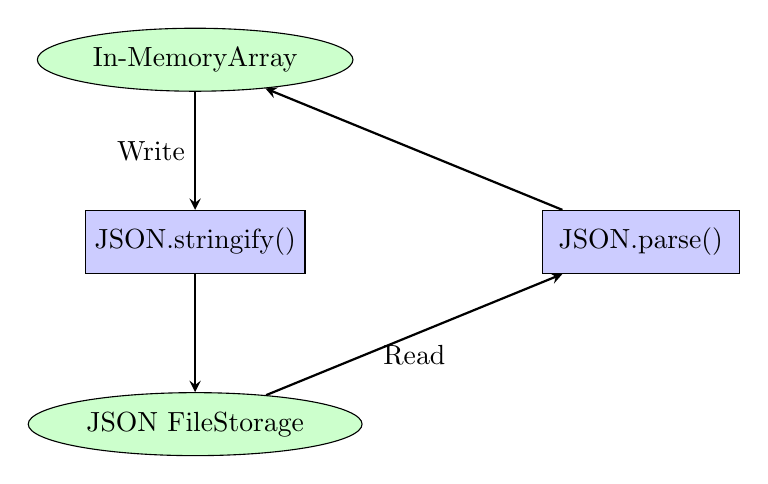
\begin{tikzpicture}[
    node distance=1.5cm,
    process/.style={rectangle, draw, fill=blue!20, minimum width=2.5cm, minimum height=0.8cm},
    data/.style={ellipse, draw, fill=green!20, minimum width=2cm, minimum height=0.8cm},
    arrow/.style={thick,->,>=stealth}
]
    \node[data] (memory) {In-Memory\\Array};
    \node[process, below=of memory] (stringify) {JSON.stringify()};
    \node[data, below=of stringify] (file) {JSON File\\Storage};
    \node[process, right=3cm of stringify] (parse) {JSON.parse()};
    
    % Arrows
    \draw[arrow] (memory) -- node[left] {Write} (stringify);
    \draw[arrow] (stringify) -- (file);
    \draw[arrow] (file) -- node[below] {Read} (parse);
    \draw[arrow] (parse) -- (memory);
\end{tikzpicture}
\caption{Data Persistence Cycle}
\end{figure}

\section{Development Workflow}

\subsection{Setup and Running}
\begin{enumerate}
    \item Install dependencies: \texttt{npm install}
    \item Start development server: \texttt{npm run dev}
    \item Server runs on port 7999 with auto-reload
    \item Test endpoints using Postman or similar tools
\end{enumerate}

\subsection{Testing Strategy}
\begin{itemize}
    \item Manual testing using Postman
    \item Create authors first, then books with author IDs
    \item Test all CRUD operations for both resources
    \item Verify error handling with invalid requests
\end{itemize}

\section{Future Enhancements}

\subsection{Potential Improvements}
\begin{itemize}
    \item Implement asynchronous file operations
    \item Add input validation and sanitization
    \item Replace file storage with database (MongoDB/PostgreSQL)
    \item Add authentication and authorization
    \item Implement pagination for large datasets
    \item Add comprehensive test suite
    \item Generate API documentation with Swagger
\end{itemize}

\section{Conclusion}

The Book Service API demonstrates a well-structured approach to building RESTful web services using modern TypeScript and Express.js. The application showcases:

\begin{itemize}
    \item Clean separation of concerns with modular architecture
    \item Consistent CRUD operation patterns
    \item Proper error handling and HTTP status codes
    \item Type safety through TypeScript interfaces
    \item Simple yet effective data persistence strategy
\end{itemize}

This foundation provides an excellent starting point for learning API development concepts and can be easily extended with additional features as requirements evolve.

\end{document}
